% !TEX encoding = UTF-8 Unicode
% !TEX TS-program = xelatex 
\begin{QUESTIONS}
    \begin{QUESTION}
        \begin{ExamInfo}{104}{學測}{單選}{1}
        \end{ExamInfo}
        \begin{ExamAnsRateInfo}{88}{99}{98}{67}
        \end{ExamAnsRateInfo}
        \begin{QBODY}
		每週同一時間點記錄某植物的成長高度, 連續五週的數據為
			${{a}_{1}}=1, {{a}_{2}}=2, {{a}_{3}}=6,{{a}_{4}}=15, {{a}_{5}}=31$
			請問此成長高度數列滿足下列選項中哪一個式子?
			\begin{QOPS}
				\QOP ${{a}_{t+1}}=3{{a}_{t}}-1,t=1,2,3,4$
				\QOP ${{a}_{t}}=t!,t=1,2,3,4,5$
				\QOP ${{a}_{t+1}}={{a}_{t}}+{{t}^{2}},t=1,2,3,4$
				\QOP ${{a}_{t}}={{2}^{t}}-1,t=1,2,3,4,5$
				\QOP ${{a}_{t+1}}=t{{a}_{t}}+1,t=1,2,3,4$
			\end{QOPS}
        \end{QBODY}
        \begin{QFROMS}
        \end{QFROMS}
        \begin{QTAGS}\QTAG{B2C1數列級數}\end{QTAGS}
        \begin{QANS}
            (3)
        \end{QANS}
        \begin{QSOLLIST}
			\begin{QSOL}
				觀察前後向的差可得 ${{a}_{t+1}}={{a}_{t}}+{{t}^{2}}$
			\end{QSOL}
        \end{QSOLLIST}
        \begin{QEMPTYSPACE}
        \end{QEMPTYSPACE}
    \end{QUESTION}
    \begin{QUESTION}
        \begin{ExamInfo}{104}{學測}{單選}{2}
        \end{ExamInfo}
        \begin{ExamAnsRateInfo}{68}{88}{72}{44}
        \end{ExamAnsRateInfo}
        \begin{QBODY}
		第 1 天獲得 1 元、第 2 天獲得 2 元、第 3 天獲得 4 元、第 4 天獲得 8 元、依此每天所獲得的錢為前一天的兩倍, 如此進行到第 30 天,試問這 30 天所獲得的錢,總數最接近下列哪一個選項?
		\begin{QOPS}
			\QOP \[10,000\] 元
			\QOP \[1,000,000\] 元
			\QOP \[100,000,000\] 元
			\QOP \[1,000,000,000\] 元
			\QOP \[1,000,000,000,000\] 元
		\end{QOPS}
        \end{QBODY}
        \begin{QFROMS}
        \end{QFROMS}
        \begin{QTAGS}\QTAG{B2C1數列級數}\end{QTAGS}
        \begin{QANS}
            (4)
        \end{QANS}
        \begin{QSOLLIST}
        \end{QSOLLIST}
        \begin{QEMPTYSPACE}
        \end{QEMPTYSPACE}
    \end{QUESTION}
    \begin{QUESTION}
        \begin{ExamInfo}{104}{學測}{單選}{3}
        \end{ExamInfo}
        \begin{ExamAnsRateInfo}{57}{78}{60}{33}
        \end{ExamAnsRateInfo}
        \begin{QBODY}
			有兩組供機器運作的配件 A、B , 其單獨發生故障的機率分別為 0.1、0.15。只有當 A, B 都發生故障時,此機器才無法運作。A、B 兩配件若用串接方式,前面故障會導致後面故障,但若後面故障則不會影響前面的故障情形;若用並列方式,則故障情形互不影響。若考慮以下三種情形:\\
			(一) 將B 串接於A之後\\
			(二) 將A串接於B 之後\\
			(三) 將A, B獨立並列\\
			在情況(一)、(二)、(三)之下, 機器無法運作的機率分別為 ${{p}_{1}}$ 、${{p}_{2}}$ 、${{p}_{3}}$ 。
			請選出正確的選項。
			\begin{QOPS}
				\QOP ${{p}_{1}}>{{p}_{2}}>{{p}_{3}}$
				\QOP ${{p}_{2}}>{{p}_{1}}>{{p}_{3}}$
				\QOP ${{p}_{3}}>{{p}_{2}}>{{p}_{1}}$
				\QOP ${{p}_{3}}>{{p}_{1}}>{{p}_{2}}$
				\QOP ${{p}_{1}}={{p}_{2}}>{{p}_{3}}$
			\end{QOPS}
        \end{QBODY}
        \begin{QFROMS}
        \end{QFROMS}
        \begin{QTAGS}\QTAG{B2C3機率}\end{QTAGS}
        \begin{QANS}
            (2)
        \end{QANS}
        \begin{QSOLLIST}
        \end{QSOLLIST}
        \begin{QEMPTYSPACE}
        \end{QEMPTYSPACE}
    \end{QUESTION}
    \begin{QUESTION}
        \begin{ExamInfo}{104}{學測}{單選}{4}
        \end{ExamInfo}
        \begin{ExamAnsRateInfo}{31}{51}{27}{15}
        \end{ExamAnsRateInfo}
        \begin{QBODY}
			一線性規劃問題的可行解區域為坐標平面上的正八邊形 ABCDEFGH 及其內部,如右圖。已知目標函數$ax+by+3$(其中 a, b 為實數)的最大值只發生在 B 點。請問當目標函數改為$3-bx-ay$ 時,最大值會發生在下列哪一點?\\
			\definecolor{light-gray}{gray}{0.75}

			%先設定好單位的大小 才有辦法產生出正確的 pspicture size
			\psset{xunit=0.6cm,yunit=0.6cm,algebraic=true,dimen=middle,dotstyle=o,dotsize=3pt 0,linewidth=0.8pt,arrowsize=3pt 2,arrowinset=0.25}

			\begin{pspicture*}(-1,-1)(9,9)
			\psaxes[labelFontSize=\scriptsize,xAxis=true,yAxis=true,Dx=1.,Dy=1.,ticksize=-2pt 0,subticks=1,labels=none,ticks=none]{->}(0,0)(-1,-1)(8,8)[$x$,0][$y$,90]
			%labelFontSize=\scriptsize

			\pspolygon*[linecolor=light-gray](2,0)(4.828,0)(6.828,2)(6.828,4.828)(4.828,6.828)(2,6.828)(0,4.828)(0,2)
			\pspolygon[linecolor=black](2,0)(4.828,0)(6.828,2)(6.828,4.828)(4.828,6.828)(2,6.828)(0,4.828)(0,2)
			\rput[t](2,-0.1){$H$}
			\rput[t](4.828,-0.1){$A$}
			\rput[l](6.928,2){$B$}
			\rput[l](6.928,4.828){$C$}
			\rput[b](4.828,6.928){$D$}
			\rput[b](2,6.928){$E$}
			\rput[r](-0.1,4.828){$F$}
			\rput[r](-0.1,2){$G$}
			\end{pspicture*}
			%%
			\\
			\begin{QOPSINONELINE}
			\QOP $A$	\QOP $B$	\QOP $C$	\QOP $D$ \QOP $E$
			\end{QOPSINONELINE}
        \end{QBODY}
        \begin{QFROMS}
        \end{QFROMS}
        \begin{QTAGS}\QTAG{B3C2直線與圓}\end{QTAGS}
        \begin{QANS}
            (1)
        \end{QANS}
        \begin{QSOLLIST}
			
        \end{QSOLLIST}
        \begin{QEMPTYSPACE}
        \end{QEMPTYSPACE}
    \end{QUESTION}
\end{QUESTIONS}
\begin{QUESTIONS}
    \begin{QUESTION}
        \begin{ExamInfo}{104}{學測}{多選}{5}
        \end{ExamInfo}
        \begin{ExamAnsRateInfo}{48}{76}{48}{20}
        \end{ExamAnsRateInfo}
        \begin{QBODY}
			小明參加某次路跑 10 公里組的比賽, 下表爲小明手錶所記錄之各公里的完成時間、平均心率及步數:
                \begin{tabular}{|c|c|c|c|}
                    \hline 
					    {}   & 完成時間  &	平均心率	& 步數  \\ \hline
					第一公里 &	5:00	 &  161	        & 990   \\ \hline
					第二公里 &	4:50	 &  162	        & 1000  \\ \hline
					第三公里 &	4:50	 &  165	        & 1005  \\ \hline
					第四公里 &	4:55	 &  162	        & 995   \\ \hline
					第五公里 &	4:40	 &  171	        & 1015  \\ \hline
					第六公里 &	4:41	 &  170	        & 1005  \\ \hline
					第七公里 &	4:35	 &  173	        & 1050  \\ \hline
					第八公里 &	4:35	 &  181	        & 1050  \\ \hline
					第九公里 &	4:40	 &  171	        & 1050  \\ \hline
					第十公里 &	4:34	 &  188	        & 1100  \\ \hline
                \end{tabular} 
			在這10公里的比賽過程,請依據上述數據,選出正確的選項。
			\begin{QOPS}
				\QOP 由每公里的平均心率得知小明最高心率爲188
				\QOP 小明此次路跑, 每步距離的平均小於1 公尺
				\QOP 每公里完成時間和每公里平均心率的相關係數爲正相關
				\QOP 每公里步數和每公里平均心率的相關係數爲正相關
				\QOP 每公里完成時間和每公里步數的相關係數爲負相關
			\end{QOPS}
        \end{QBODY}
        \begin{QFROMS}
        \end{QFROMS}
        \begin{QTAGS}\QTAG{B2C4數據分析}\end{QTAGS}
        \begin{QANS}
            (2)(4)(5)
        \end{QANS}
        \begin{QSOLLIST}
        \end{QSOLLIST}
        \begin{QEMPTYSPACE}
        \end{QEMPTYSPACE}
    \end{QUESTION}
    \begin{QUESTION}
        \begin{ExamInfo}{104}{學測}{多選}{6}
        \end{ExamInfo}
        \begin{ExamAnsRateInfo}{45}{74}{43}{18}
        \end{ExamAnsRateInfo}
        \begin{QBODY}
			若 $f\left( x \right)$ 是首項係數為 $1$ 的實係數二次多項式。請選出正確的選項。
			\begin{QOPS}
				\QOP 若 $f\left( 2 \right)=0$,則 $x-2$ 可整除 $f\left( x \right)$
				\QOP 若 $f\left( 2 \right)=0$,則 $f\left( x \right)$ 為整係數多項式
				\QOP 若 $f\left( \sqrt{2} \right)=0$,則 $f\left( -\sqrt{2} \right)=0$
				\QOP 若 $f\left( 2i \right)=0$,則 $f\left( -2i \right)=0$
				\QOP 若 $f\left( 2i \right)=0$,則 $f\left( x \right)$ 為整係數多項式
			\end{QOPS}
        \end{QBODY}
        \begin{QFROMS}
        \end{QFROMS}
        \begin{QTAGS}\QTAG{B1C2多項式函數}\end{QTAGS}
        \begin{QANS}
            (1)(4)(5)
        \end{QANS}
        \begin{QSOLLIST}
        \end{QSOLLIST}
        \begin{QEMPTYSPACE}
        \end{QEMPTYSPACE}
    \end{QUESTION}
    \begin{QUESTION}
        \begin{ExamInfo}{104}{學測}{多選}{7}
        \end{ExamInfo}
        \begin{ExamAnsRateInfo}{67}{92}{77}{32}
        \end{ExamAnsRateInfo}
        \begin{QBODY}
			坐標平面上,在函數圖形 $y={{2}^{x}}$ 上,標示 $A$、$B$、$C$、$D$ 四個點,其 $x$ 座標分別為 $-1$、$0$、$1$、$2$。請選出正確的選項。
			\begin{QOPS}
				\QOP 點 $B$ 落在直線 $AC$ 的下方
				\QOP 在直線 $AB$、直線 $BC$ 、直線 $CD$ 中,以直線 $CD$ 的斜率最大
				\QOP $A$、$B$、$C$、$D$ 四個點,以點 $B$ 最靠近 $x$ 軸
				\QOP 直線 $y=2x$ 與 $y={{2}^{x}}$ 的圖形有兩個交點
				\QOP 點 $A$ 與點 $C$ 對稱於 $y$ 軸
			\end{QOPS}
        \end{QBODY}
        \begin{QFROMS}
        \end{QFROMS}
        \begin{QTAGS}\QTAG{B1C3指對數函數}\end{QTAGS}
        \begin{QANS}
            (1)(2)(4)
        \end{QANS}
        \begin{QSOLLIST}
			\begin{QSOL}
				%先設定好單位的大小 才有辦法產生出正確的 pspicture size
				\psset{xunit=1cm,yunit=1cm,algebraic=true,dimen=middle,dotstyle=o,dotsize=3pt 0,linewidth=0.8pt,arrowsize=3pt 2,arrowinset=0.25}
				\begin{pspicture*}(-1.5,-0.5)(4,6)
				\psaxes[labelFontSize=\scriptsize, xAxis=true,yAxis=true,Dx=1.,Dy=1.,ticksize=-2pt]{->}(0,0)(-1.5,-0.5)(3,5)[$x$,0][$y$,90]
				%labelFontSize=\scriptsize

				\psplot[plotpoints=200]{-1.5}{2.2}{2^x}
				\psplot[plotpoints=200]{-0.2}{2.2}{2*x}


				%\begin{scriptsize}

				\rput[br](2,4.3){$y=2^x $}
				\rput[l](0.35,0.5){$y=2x $}


				%\psline[linestyle=dashed](-1,0.5)(0.,1.)
				%\psline[linestyle=dashed](0.,1)(1.,2.)
				%\psline[linestyle=dashed](1.,2)(2.,4.)


				\psdots[dotstyle=*](-1,0.5)
				\rput[lt](-1,0.4){$A$}
				\psdots[dotstyle=*](0.,1.)
				\rput[lt](0,0.9){$B$}
				\psdots[dotstyle=*](1.,2.)
				\rput[lt](1,1.9){$C$}
				\psdots[dotstyle=*](2.,4.)
				\rput[lt](2,3.9){$D$}


				%\end{scriptsize}
				\end{pspicture*}
			\end{QSOL}
        \end{QSOLLIST}
        \begin{QEMPTYSPACE}
        \end{QEMPTYSPACE}
    \end{QUESTION}
    \begin{QUESTION}
        \begin{ExamInfo}{104}{學測}{多選}{8}
        \end{ExamInfo}
        \begin{ExamAnsRateInfo}{48}{71}{49}{24}
        \end{ExamAnsRateInfo}
        \begin{QBODY}
			坐標平面上有一雙曲線,其漸近線為 $x-y=0$ 和 $x+y=0$。關於此雙曲線的性質,請選出正確的選項。
			\begin{QOPS}
				\QOP 此雙曲線的方程式為 $\frac{{{x}^{2}}}{{{r}^{2}}}-\frac{{{y}^{2}}}{{{r}^{2}}}=1$ 或 $\frac{{{x}^{2}}}{{{r}^{2}}}-\frac{{{y}^{2}}}{{{r}^{2}}}=-1$,其中 $r$ 為非零實數
				\QOP 此雙曲線的貫軸長等於共軛軸長
				\QOP 若點 $\left( a,b \right)$ 為此雙曲線在第一象限上一點,則當 $a>1000$ 時,$\left| a-b \right|<1$
				\QOP 若點 $\left( a,b \right),\ \left( a',b' \right)$ 為此雙曲線在第一象限上兩點且 $a>a'$,則 $b<b'$
				\QOP 此雙曲線同時對稱於 $x$ 軸 與 $y$ 軸
			\end{QOPS}
        \end{QBODY}
        \begin{QFROMS}
        \end{QFROMS}
        \begin{QTAGS}\QTAG{B4C4二次曲線}\end{QTAGS}
        \begin{QANS}
            (1)(2)(4)(5)
        \end{QANS}
        \begin{QSOLLIST}
        \end{QSOLLIST}
        \begin{QEMPTYSPACE}
        \end{QEMPTYSPACE}
    \end{QUESTION}
    \begin{QUESTION}
        \begin{ExamInfo}{104}{學測}{多選}{9}
        \end{ExamInfo}
        \begin{ExamAnsRateInfo}{49}{77}{45}{25}
        \end{ExamAnsRateInfo}
        \begin{QBODY}
				如圖,以 $M$ 為圓心、$\overline{MA}=8$ 為半徑畫圓,$\overline{AE}$ 為該圓的直徑,$B$、$C$、$D$ 三點皆在圓上,且 $\overline{AB}=\overline{BC}=\overline{CD}=\overline{DE}$。若 $\lvec{MD}\,=8\left( \cos \left( \theta +90{}^\circ  \right),\sin \left( \theta +90{}^\circ  \right) \right)$。請選出正確的選項。
			\begin{QOPS}
				\QOP $\lvec{MA}\,=8\left( \cos \theta ,\sin \theta  \right)$
				\QOP $\lvec{MC}\,=8\left( \cos \left( \theta +45{}^\circ  \right),\sin \left( \theta +45{}^\circ  \right) \right)$
				\QOP (內積) $\lvec{MA}\,\cdot \lvec{MA}\,=8$
				\QOP (內積) $\lvec{MB}\,\cdot \lvec{MD}\,=0$
				\QOP $\lvec{BD}\,=\left( 8\cos \theta +\cos \left( \theta +90{}^\circ  \right),\sin \theta +\cos \left( \theta +90{}^\circ  \right) \right)$
			\end{QOPS}
			
			%先設定好單位的大小 才有辦法產生出正確的 pspicture size
			\psset{xunit=1cm,yunit=1cm,algebraic=true,dimen=middle,dotstyle=o,dotsize=3pt 0,linewidth=0.8pt,arrowsize=3pt 2,arrowinset=0.25}
			\def\CRadiusOffset{3.3}
			\def\CRadius{3}
			% 設定整張圖片的大小
			\begin{pspicture*}(-4,-1)(4,4) 

			%設定軸
			\psaxes[labelFontSize=\scriptsize, xAxis=false,yAxis=false,Dx=1.,Dy=1.,ticksize=-2pt]{->}(0,0)(-4,-1)(4,4) %[$x$,0][$y$,90]
			\pswedge[fillstyle=solid]{\CRadius}{15}{195}

			%可畫方程式


			%設定文字圖標等

			\psdots[dotstyle=*](0,0)
			\rput[t](0,-0.2){$M$}
			\psdots[dotstyle=*](\CRadius;15)
			\rput(\CRadiusOffset;15){$A$}
			\psdots[dotstyle=*](\CRadius;60)
			\rput(\CRadiusOffset;60){$B$}
			\psdots[dotstyle=*](\CRadius;105)
			\rput(\CRadiusOffset;105){$C$}
			\psdots[dotstyle=*](\CRadius;150)
			\rput(\CRadiusOffset;150){$D$}
			\psdots[dotstyle=*](\CRadius;195)
			\rput(\CRadiusOffset;195){$E$}
			\end{pspicture*}
        \end{QBODY}
        \begin{QFROMS}
        \end{QFROMS}
        \begin{QTAGS}\QTAG{B3C3平面向量}\end{QTAGS}
        \begin{QANS}
            (2)(4)
        \end{QANS}
        \begin{QSOLLIST}
        \end{QSOLLIST}
        \begin{QEMPTYSPACE}
        \end{QEMPTYSPACE}
    \end{QUESTION}
    \begin{QUESTION}
        \begin{ExamInfo}{104}{學測}{多選}{10}
        \end{ExamInfo}
        \begin{ExamAnsRateInfo}{45}{64}{42}{29}
        \end{ExamAnsRateInfo}
        \begin{QBODY}
			某一班共有 $45$ 人, 問卷調查有手機與平板電腦的人數。從統計資料顯示此班有 $35$ 人有手機, 而有24 人有平板電腦。設:\\
				$A$ 為同時有手機與平板電腦的人數\\
				$B$ 為有手機,但沒有平板電腦的人數\\
				$C$ 為沒有手機,但有平板電腦的人數\\
				$D$ 為沒有手機,也沒有平板電腦的人數\\
			請選出恆成立的不等式選項。
			\begin{QOPSINONELINE}
				\QOP $A>B$	\QOP $A>C$	\QOP $B>C$	\QOP $B>D$	\QOP $C>D$
			\end{QOPSINONELINE}

        \end{QBODY}
        \begin{QFROMS}
        \end{QFROMS}
        \begin{QTAGS}\QTAG{B2C2排列組合}\end{QTAGS}
        \begin{QANS}
            (2)(3)(4)
        \end{QANS}
        \begin{QSOLLIST}
			\begin{QSOL}
			\end{QSOL}
        \end{QSOLLIST}
        \begin{QEMPTYSPACE}
        \end{QEMPTYSPACE}
    \end{QUESTION}
\end{QUESTIONS}
\begin{QUESTIONS}
    \begin{QUESTION}
        \begin{ExamInfo}{104}{學測}{填充}{A}
        \end{ExamInfo}
        \begin{ExamAnsRateInfo}{43}{81}{44}{4}
        \end{ExamAnsRateInfo}
        \begin{QBODY}
			如圖,老王在平地點 $A$ 測得遠方山頂點 $P$  的仰角為 $13{}^\circ $。老王朝著山的方向前進 $37$ 公丈後來到點 $B$ , 再測得山頂點 $P$ 的仰角為 $15{}^\circ $。則山高約為$\TCNBOX{\TCN\TCN}$公丈。(四捨五入至個位數, $\tan 13{}^\circ \approx 0.231$, $\tan 15{}^\circ \approx 0.268$)
			
			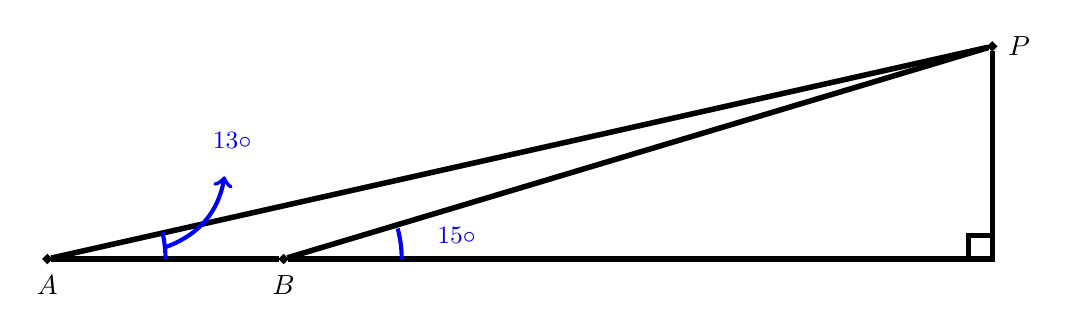
\begin{tikzpicture}[line width=2pt, scale=1.5] 
			\node (vO) at (0,0) {};
			\draw (0,0) rectangle (-.2,.2);
			\foreach \n/\l\x/\y  in {A/-90/-8/0, B/-90/-6/0, P/0/0/1.8}{
					\node[label=\l:$\n$, draw, inner sep=0pt, circle,fill] (v\n) at (\x,\y)  {};
			}
			\foreach \x/\y in {A/B, B/O, O/P, P/B, P/A}{
					\draw (v\x) to (v\y);
			}
			\draw[blue, line width=1.5pt] (-5,0) arc [start angle = 0, end angle =15, radius=1cm];
			\node[right, blue] at (-4.8,0.2) {\small $15\circ$};
			\node[right, blue] at (-6.7,1) {\small $13\circ$};
			\draw[->, line width=1.5pt, blue] (-7,0.1) to[bend right] (-6.5,0.7);
			\draw[blue, line width=1.5pt] (-7,0) arc [start angle = 0, end angle =13, radius=1cm];
			\end{tikzpicture}

        \end{QBODY}
        \begin{QFROMS}
        \end{QFROMS}
        \begin{QTAGS}\QTAG{B3C1三角}\end{QTAGS}
        \begin{QANS}
            $62$
        \end{QANS}
        \begin{QSOLLIST}
        \end{QSOLLIST}
        \begin{QEMPTYSPACE}
        \end{QEMPTYSPACE}
    \end{QUESTION}
    \begin{QUESTION}
        \begin{ExamInfo}{104}{學測}{填充}{B}
        \end{ExamInfo}
        \begin{ExamAnsRateInfo}{39}{64}{35}{18}
        \end{ExamAnsRateInfo}
        \begin{QBODY}
				不透明袋中有 $3$ 白 $3$ 紅共 $6$ 個球,球大小形狀相同,僅顏色相異。甲、乙、丙、丁、戊 $5$人依甲第一、乙第二、… …、戊第五的次序,從袋中各取一球,取後不放回。試問在甲、乙取出不同色球的條件下,戊取得紅球的機率為$\TCNBOX{\FR{\TCN}{\TCN}}$。( 化為最簡分數)
        \end{QBODY}
        \begin{QFROMS}
        \end{QFROMS}
        \begin{QTAGS}\QTAG{B2C3機率}\end{QTAGS}
        \begin{QANS}
            $\dfrac{1}{2}$
        \end{QANS}
        \begin{QSOLLIST}
        \end{QSOLLIST}
        \begin{QEMPTYSPACE}
        \end{QEMPTYSPACE}
    \end{QUESTION}
    \begin{QUESTION}
        \begin{ExamInfo}{104}{學測}{填充}{C}
        \end{ExamInfo}
        \begin{ExamAnsRateInfo}{21}{49}{11}{3}
        \end{ExamAnsRateInfo}
        \begin{QBODY}
			小燦預定在陽台上種植玫瑰、百合、菊花和向日葵等四種盆栽。如果陽台上的空間最多能種 $8$ 盆,可以不必擺滿,並且每種花至少一盆,則小燦買盆栽的方法共有$\TCNBOX{\TCN\TCN}$種。
        \end{QBODY}
        \begin{QFROMS}
        \end{QFROMS}
        \begin{QTAGS}\QTAG{B2C2排列組合}\end{QTAGS}
        \begin{QANS}
            $70$
        \end{QANS}
        \begin{QSOLLIST}
        \end{QSOLLIST}
        \begin{QEMPTYSPACE}
        \end{QEMPTYSPACE}
    \end{QUESTION}
    \begin{QUESTION}
        \begin{ExamInfo}{104}{學測}{填充}{D}
        \end{ExamInfo}
        \begin{ExamAnsRateInfo}{13}{36}{3}{0}
        \end{ExamAnsRateInfo}
        \begin{QBODY}
			平面 $x-y+z=0$ 與三平面 $x=2,\ x-y=-2,\ x+y=2$ 分別相交所得的三直線可圍成一三角形。此三角形之周長化成最簡根式,可表為 $a\sqrt{b}+c\sqrt{d}$,其中 $a,b,c,d$ 為正整數且 $b<d$,則 $a=\TCNBOX{\TCN },\ b=\TCNBOX{\TCN },\ c=\TCNBOX{\TCN },\ d=\TCNBOX{\TCN }$。
        \end{QBODY}
        \begin{QFROMS}
        \end{QFROMS}
        \begin{QTAGS}\QTAG{B4C1空間向量}\end{QTAGS}
        \begin{QANS}
            $6 \sqrt{2} + 2\sqrt{6}$
        \end{QANS}
        \begin{QSOLLIST}
			\begin{QSOL}
			已知 $x=2,\ x-y=-2,\ x+y=2$ 皆缺 $z$ 項
			可先找到此三平面在 $xy$ 平面上所形成之三角形,在投影至 $x-y+z=0$ 平面上。
			$\left\{ \begin{aligned}
			  & x=2 \\ 
			 & x-y=-2 \\ 
			\end{aligned} \right.\Rightarrow \left\{ \begin{aligned}
			  & x=2 \\ 
			 & y=4 \\ 
			\end{aligned} \right.\Rightarrow \left( 2,4 \right)$; $\left\{ \begin{aligned}
			  & x-y=-2 \\ 
			 & x+y=2 \\ 
			\end{aligned} \right.\Rightarrow \left\{ \begin{aligned}
			  & x=0 \\ 
			 & y=2 \\ 
			\end{aligned} \right.\Rightarrow \left( 0,2 \right)$;$\left\{ \begin{aligned}
			  & x+y=2 \\ 
			 & x=2 \\ 
			\end{aligned} \right.\Rightarrow \left\{ \begin{aligned}
			  & x=2 \\ 
			 & y=0 \\ 
			\end{aligned} \right.\Rightarrow \left( 2,0 \right)$
			再代入$x-y+z=0$ 可得三角形三頂點:$\left( 2,4,2 \right)$、$\left( 0,2,2 \right)$、$\left( 2,0,-2 \right)$
			計算三角形周長 $\sqrt{{{2}^{2}}+{{2}^{2}}}+\sqrt{{{\left( -2 \right)}^{2}}+{{2}^{2}}+{{4}^{2}}}+\sqrt{{{4}^{2}}+{{4}^{2}}}=2\sqrt{2}+2\sqrt{6}+4\sqrt{2}=6\sqrt{2}+2\sqrt{6}$
			\end{QSOL}
        \end{QSOLLIST}
        \begin{QEMPTYSPACE}
        \end{QEMPTYSPACE}
    \end{QUESTION}
    \begin{QUESTION}
        \begin{ExamInfo}{104}{學測}{填充}{E}
        \end{ExamInfo}
        \begin{ExamAnsRateInfo}{31}{71}{21}{1}
        \end{ExamAnsRateInfo}
        \begin{QBODY}
			坐標平面上,直線 ${{L}_{1}}$ 與 ${{L}_{2}}$ 的方程式分別為 $x+2y=0$ 與 $3x-5y=0$。為了確定平面上某一定點 $P$ 的坐標,從 ${{L}_{1}}$ 上的一點 ${{Q}_{1}}$ 偵測得向量 $\overset{\rightharpoonup }{\mathop{{{Q}_{1}}P}}\,=\left( -7,9 \right)$,再從 ${{L}_{2}}$ 上的點 ${{Q}_{2}}$ 偵測得向量 $\overset{\rightharpoonup }{\mathop{{{Q}_{2}}P}}\,=\left( -6,-8 \right)$,則 $P$ 點的坐標為 $\TCNBOX{\left( \TCN, \TCN \right)}$。
        \end{QBODY}
        \begin{QFROMS}
        \end{QFROMS}
        \begin{QTAGS}\QTAG{B3C3平面向量}\end{QTAGS}
        \begin{QANS}
            $(9,1)$
        \end{QANS}
        \begin{QSOLLIST}
			\begin{QSOL}
				設 $P\left( a,b \right)$ 則 ${{Q}_{1}}\left( a+7,\ b-9 \right)$、${{Q}_{2}}\left( a+6,\ b+8 \right)$\\
				且 ${{Q}_{1}}\in x+2y=0,\ {{Q}_{2}}\in 3x-5y=0$
				$\Rightarrow \left\{ \begin{aligned}
				  & a+7+2b-18=0 \\ 
				 & 3a+18-5b-40=0 \\ 
				\end{aligned} \right.$$\Rightarrow \left\{ \begin{aligned}
				  & a+2b=11 \\ 
				 & 3a-5b=22 \\ 
				\end{aligned} \right.\Rightarrow \left( a,\ b \right)=\left( 9,\ 1 \right)$

			\end{QSOL}
        
			\begin{QSOL}
				 幾何意義:可觀察得 $x+2y=0$ 與 $3x-5y=0$ 交於 $\left( 0,\ 0 \right)$
				  由題意『從 ${{L}_{1}}$ 上的一點 ${{Q}_{1}}$ 偵測得向量 $\lvec{{Q}_{1}P}\,=\left( -7,9 \right)$』
				  $\Rightarrow $可得 $P$ 在與 ${{L}_{1}}$ 平行且過 $\left( -7,9 \right)$的直線上, $P\in x+2y=11$
				  由題意『再從 ${{L}_{2}}$ 上的點 ${{Q}_{2}}$ 偵測得向量 $\lvec{{Q}_{2}P}\,=\left( -6,-8 \right)$』
				  $\Rightarrow $可得 $P$ 在與 ${{L}_{2}}$ 平行的直線上,且過 $\left( -6,-8 \right)$ $P\in 3x-5y=22$
				  可解$\left\{ \begin{aligned}
				  & x+2y=11 \\ 
				 & 3x-5y=22 \\ 
				\end{aligned} \right.\Rightarrow P\left( 9,\ 1 \right)$
			\end{QSOL}
        \end{QSOLLIST}
        \begin{QEMPTYSPACE}
        \end{QEMPTYSPACE}
    \end{QUESTION}
    \begin{QUESTION}
        \begin{ExamInfo}{104}{學測}{填充}{F}
        \end{ExamInfo}
        \begin{ExamAnsRateInfo}{26}{57}{18}{3}
        \end{ExamAnsRateInfo}
        \begin{QBODY}
			小華準備向銀行貸款 $3$ 百萬元當做創業基金,其年利率爲$3\%$,約定三年期滿一次還清貸款的本利和。銀行貸款一般以複利( 每年複利一次)計息還款,但給小華創業優惠改以單利計息還款。試問在此優惠下, 小華在三年期滿還款時可以比一般複利計息少繳$\TCNBOX{\TCN\TCN\TCN\TCN }$元。
        \end{QBODY}
        \begin{QFROMS}
        \end{QFROMS}
        \begin{QTAGS}\QTAG{B1C3指對數函數}\end{QTAGS}
        \begin{QANS}
            $8181$
        \end{QANS}
        \begin{QSOLLIST}
        \end{QSOLLIST}
        \begin{QEMPTYSPACE}
        \end{QEMPTYSPACE}
    \end{QUESTION}
    \begin{QUESTION}
        \begin{ExamInfo}{104}{學測}{填充}{G}
        \end{ExamInfo}
        \begin{ExamAnsRateInfo}{46}{81}{47}{10}
        \end{ExamAnsRateInfo}
        \begin{QBODY}
			某一公司, 有 A、B、C 三個營業據點, 開始時各有36 位營業員, 為了讓營業員了解各據點業務狀況, 所以進行兩次調動。每次調動都是:\\
			將當時A 據點營業員中的1/6 調到B 據點、1/6 調到C 據點;\\
			將當時B 據點營業員中的1/6 調到A 據點、1/3 調到C 據點;\\
			將當時C 據點營業員中的1/6 調到A 據點、1/6 調到B 據點。\\
			則兩次的調動後, C 據點有 $\TCNBOX{\TCN\TCN}$ 位營業員。

        \end{QBODY}
        \begin{QFROMS}
        \end{QFROMS}
        \begin{QTAGS}\QTAG{B4C3矩陣}\end{QTAGS}
        \begin{QANS}
            $44$
        \end{QANS}
        \begin{QSOLLIST}
        \end{QSOLLIST}
        \begin{QEMPTYSPACE}
        \end{QEMPTYSPACE}
    \end{QUESTION}
    \begin{QUESTION}
        \begin{ExamInfo}{104}{學測}{填充}{H}
        \end{ExamInfo}
        \begin{ExamAnsRateInfo}{43}{77}{41}{11}
        \end{ExamAnsRateInfo}
        \begin{QBODY}
		有一底面為正方形的四角錐, 其展開圖如下圖所示, 其中兩側面的三角形邊長為 $3,\ 4,\ 5$,則此角錐的體積為$\TCNBOX{\frac{\TCN\TCN\sqrt{\TCN}}{3}}$。(化成最簡根式) 
		
		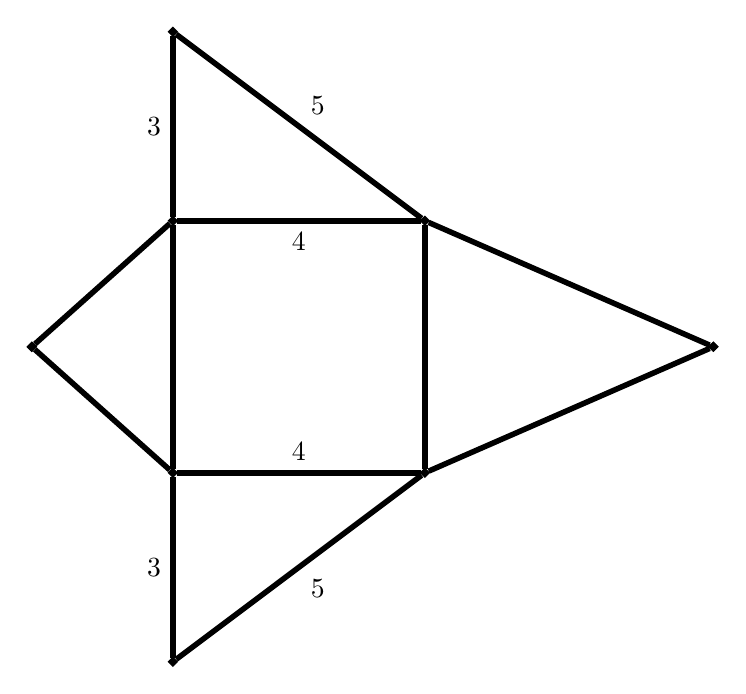
\begin{tikzpicture}[line width=2pt, scale=0.8]
			\foreach \n/\x/\y in {A/-2/2,B/2/2,C/-2/5,D/6.58/0,E/-4.24/0}{
					\node[inner sep=0pt,fill, draw, circle] (v\n) at (\x, \y) {};
					\node[inner sep=0pt,fill, draw, circle] (u\n) at (\x, -\y) {};
			}
			\foreach \x/\y/\l in {B/A/4,A/E/,A/C/3,C/B/5,B/D/}{
					\draw (v\x) to node[auto] {$\l$} (v\y);
			}
			\foreach \x/\y/\l in {A/B/4,A/E/,C/A/3,B/C/5,B/D/}{
					\draw (u\x) to node[auto] {$\l$}  (u\y);
			}
			\foreach \x/\y in {uA/vA,uB/vB}{
					\draw (\x) to (\y);
			}
		\end{tikzpicture}

        \end{QBODY}
        \begin{QFROMS}
        \end{QFROMS}
        \begin{QTAGS}\QTAG{B4C1空間向量}\end{QTAGS}
        \begin{QANS}
            $\dfrac{16\sqrt{5}}{3}$
        \end{QANS}
        \begin{QSOLLIST}
        \end{QSOLLIST}
        \begin{QEMPTYSPACE}
        \end{QEMPTYSPACE}
    \end{QUESTION}
    \begin{QUESTION}
        \begin{ExamInfo}{104}{學測}{填充}{I}
        \end{ExamInfo}
        \begin{ExamAnsRateInfo}{13}{33}{6}{0}
        \end{ExamAnsRateInfo}
        \begin{QBODY}
			在空間中, 一個斜面的「坡度」定義為斜面與水平面夾角 $\theta $ 的正切值 $\tan \theta $ 。若一金字塔( 底部為一正方形, 四個斜面為等腰三角形)的每一個斜面的坡度皆為$\frac{\ 2\ }{5}$,如圖。則相鄰斜面的夾角的餘弦函數的絕對值為$\TCNBOX{\frac{\TCN\TCN}{\TCN\TCN}}$。(化成最簡分數)
			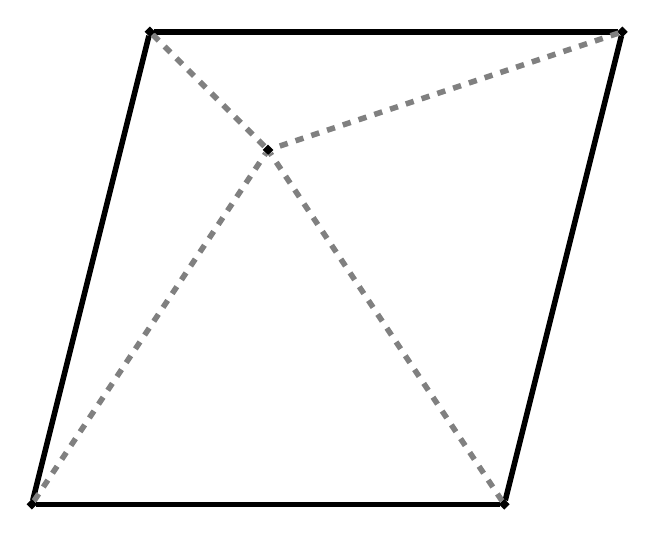
\begin{tikzpicture}[line width=2pt, scale=1.5]
				\foreach \n/\x/\y in {A/-2/-2,B/-1/2,C/3/2,D/2/-2,E/0/1}{
						\node[inner sep=0pt,fill, draw, circle]  (v\n) at  (\x,\y) {};
				}
				\foreach \x/\y in {A/B,B/C,C/D,D/A}{
						\draw (v\x) to (v\y);
						\draw[gray,dashed] (v\x) to (vE);
				}
			\end{tikzpicture}
        \end{QBODY}
        \begin{QFROMS}
        \end{QFROMS}
        \begin{QTAGS}\QTAG{B4C1空間向量}\end{QTAGS}
        \begin{QANS}
            $\dfrac{25}{29}$
        \end{QANS}
        \begin{QSOLLIST}
        \end{QSOLLIST}
        \begin{QEMPTYSPACE}
        \end{QEMPTYSPACE}
    \end{QUESTION}
    \begin{QUESTION}
        \begin{ExamInfo}{104}{學測}{填充}{J}
        \end{ExamInfo}
        \begin{ExamAnsRateInfo}{32}{71}{23}{2}
        \end{ExamAnsRateInfo}
        \begin{QBODY}
		下圖為汽車迴轉示意圖。汽車迴轉時,將方向盤轉動到極限,以低速讓汽車進行轉向圓周運動,汽車轉向時所形成的圓周的半徑就是迴轉半徑,如圖中的 $\overline{BC}$ 即是。已知在低速前進時,圖中$A$  處的輪胎行進方向與 $\overline{AC}$ 垂直, $B$ 處的輪胎行進方向與 $\overline{BC}$ 垂直。在圖中, 已知軸距 $AB$ 為 2.85 公尺,方向盤轉到極限時,輪子方向偏了 $28$ 度, 試問此車的迴轉半徑 $\overline{BC}$ 為$\TCNBOX{\TCN.\TCN}$ 公尺。( 小數點後第一位以下四捨五入,$\sin 28{}^\circ \approx 0.4695,\ \cos 28{}^\circ \approx 0.8829$)
		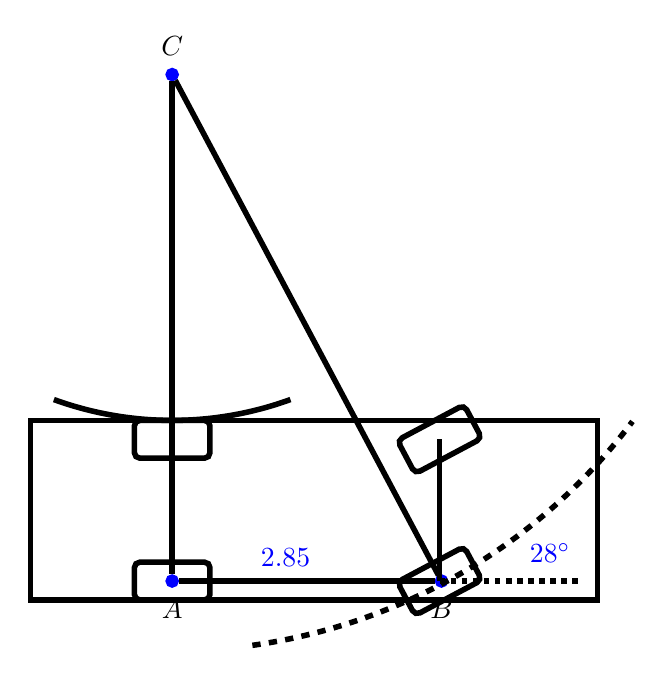
\begin{tikzpicture}[line width=2pt,scale=1.2]
			\foreach \n/\x/\y/\l in {A/0/0/270, B/2.85/0/270, C/0/5.36/90}{
					\node[label=\l:$\n$, draw, fill, inner sep=1pt, circle, blue] (v\n) at (\x,\y) {};
			}
			\draw (-1.5,-0.2) rectangle(4.5,1.7);
			\draw (2.83,0) to(2.83,1.5);
			\draw[dotted] (2.83,0) to(4.3,0);
			\node[blue] at (4,0.3) {$28^\circ$};
			\node[blue] at (1.2,0.25) {$2.85$};
			\draw[rounded corners=2pt] (-0.4,-0.2) rectangle (0.4,0.2);
			\begin{scope}[yshift=1.5cm]
			\draw[rounded corners=2pt] (-0.4,-0.2) rectangle (0.4,0.2);
			\end{scope}
			\begin{scope}[xshift=2.83cm, yshift=1.5cm]
			\draw[rounded corners=2pt, rotate=28] (-0.4,-0.2) rectangle (0.4,0.2);
			\end{scope}
			\begin{scope}[xshift=2.83cm, yshift=0cm]
			\draw[rounded corners=2pt, rotate=28] (-0.4,-0.2) rectangle (0.4,0.2);
			\end{scope}
			\foreach \x/\y in{A/B,B/C,C/A}
					\draw (v\x) to (v\y);
			\begin{scope} [yshift=5.36cm]
					\draw (250:3.66) arc [start angle =250, end angle= 290, radius =3.66cm];
					\draw[dashed] (278:6.1) arc [start angle =278, end angle= 323, radius =6.1cm];
			\end{scope}
		\end{tikzpicture}
        \end{QBODY}
        \begin{QFROMS}
        \end{QFROMS}
        \begin{QTAGS}\QTAG{B3C1三角}\end{QTAGS}
        \begin{QANS}
            $6.1$
        \end{QANS}
        \begin{QSOLLIST}
        \end{QSOLLIST}
        \begin{QEMPTYSPACE}
        \end{QEMPTYSPACE}
    \end{QUESTION}
\end{QUESTIONS}
